\chapter{Project: A Robot}\label{robot}

\epigraphhead[30]{
\epigraph{\hspace*{-.1cm}\itshape``[...] the question of whether Machines Can Think [...] is about as relevant as the question of whether Submarines Can Swim.''}%
{---Edsger Dijkstra, The Threats to Computing Science}
}\index{artificial intelligence}\index{Dijkstra, Edsger}\index{project chapter}\index{reading code}\index{writing code}

In ``project'' chapters, I'll stop pummeling you with new theory for a brief moment, and instead we'll work through a program together. Theory is necessary to learn to program, but reading and understanding actual programs is just as important.

Our project in this chapter is to build an \index{automaton}automaton, a little program that performs a task in a \index{virtual world}virtual world. Our automaton will be a mail-delivery \index{robot}robot picking up and dropping off parcels.

\section{Meadowfield}\index{roads array}

The village of \index{Meadowfield}Meadowfield isn't very big. It consists of 11 places with 14 roads between them. It can be described with this array of roads:

\begin{lstlisting}
const roads = [
  "Alice's House-Bob's House",   "Alice's House-Cabin",
  "Alice's House-Post Office",   "Bob's House-Town Hall",
  "Daria's House-Ernie's House", "Daria's House-Town Hall",
  "Ernie's House-Grete's House", "Grete's House-Farm",
  "Grete's House-Shop",          "Marketplace-Farm",
  "Marketplace-Post Office",     "Marketplace-Shop",
  "Marketplace-Town Hall",       "Shop-Town Hall"
];
\end{lstlisting}
\noindent

\vskip 1.5ex
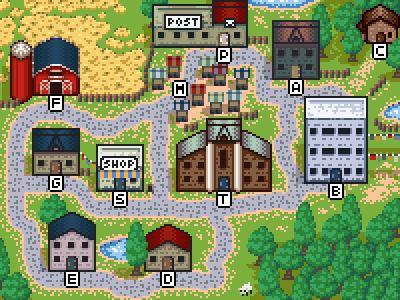
\includegraphics[width=10cm]{img/village2x.png}
\vskip 1.5ex

The network of roads in the village forms a \emph{\index{graph}graph}. A graph is a collection of points (places in the village) with lines between them (roads). This graph will be the world that our robot moves through.\index{roadGraph object}

The array of strings isn't very easy to work with. What we're interested in is the destinations that we can reach from a given place. Let's convert the list of roads to a data structure that, for each place, tells us what can be reached from there.

\begin{lstlisting}
function buildGraph(edges) {
  let graph = Object.create(null);
  function addEdge(from, to) {
    if (graph[from] == null) {
      graph[from] = [to];
    } else {
      graph[from].push(to);
    }
  }
  for (let [from, to] of edges.map(r => r.split("-"))) {
    addEdge(from, to);
    addEdge(to, from);
  }
  return graph;
}

const roadGraph = buildGraph(roads);
\end{lstlisting}
\noindent

Given an array of edges, \lstinline`buildGraph` creates a map object that, for each node, stores an array of connected nodes.\index{split method}

It uses the \lstinline`split` method to go from the road strings, which have the form \lstinline`"Start-End"`, to two-element arrays containing the start and end as separate strings.

\section{The task}

Our \index{robot}robot will be moving around the village. There are parcels in various places, each addressed to some other place. The robot picks up parcels when it comes to them and delivers them when it arrives at their destinations.

The automaton must decide, at each point, where to go next. It has finished its task when all parcels have been delivered.\index{simulation}\index{virtual world}

To be able to simulate this process, we must define a virtual world that can describe it. This model tells us where the robot is and where the parcels are. When the robot has decided to move somewhere, we need to update the model to reflect the new situation.\index{state!in!objects}

If you're thinking in terms of \index{object-oriented programming}object-oriented programming, your first impulse might be to start defining objects for the various elements in the world: a \index{class}class for the robot, one for a parcel, maybe one for places. These could then hold properties that describe their current \index{state}state, such as the pile of parcels at a location, which we could change when updating the world.

This is wrong.

At least, it usually is. The fact that something sounds like an object does not automatically mean that it should be an object in your program. Reflexively writing classes for every concept in your application tends to leave you with a collection of interconnected objects that each have their own internal, changing state. Such programs are often hard to understand and thus easy to break.\index{state!in!objects}

Instead, let's condense the village's state down to the minimal set of values that define it. There's the robot's current location and the collection of undelivered parcels, each of which has a current location and a destination address. That's it.\index{VillageState class}\index{persistent data structure}

And while we're at it, let's make it so that we don't \emph{change} this state when the robot moves but rather compute a \emph{new} state for the situation after the move.

\begin{lstlisting}
class VillageState {
  constructor(place, parcels) {
    this.place = place;
    this.parcels = parcels;
  }

  move(destination) {
    if (!roadGraph[this.place].includes(destination)) {
      return this;
    } else {
      let parcels = this.parcels.map(p => {
        if (p.place != this.place) return p;
        return {place: destination, address: p.address};
      }).filter(p => p.place != p.address);
      return new VillageState(destination, parcels);
    }
  }
}
\end{lstlisting}
\noindent

The \lstinline`move` method is where the action happens. It first checks whether there is a road going from the current place to the destination, and if not, it returns the old state since this is not a valid move.\index{map method}\index{filter method}

Then it creates a new state with the destination as the robot's new place. But it also needs to create a new set of parcels—parcels that the robot is carrying (that are at the robot's current place) need to be moved along to the new place. And parcels that are addressed to the new place need to be delivered—that is, they need to be removed from the set of undelivered parcels. The call to \lstinline`map` takes care of the moving, and the call to \lstinline`filter` does the delivering.

Parcel objects aren't changed when they are moved but re-created. The \lstinline`move` method gives us a new village state but leaves the old one entirely intact.

\begin{lstlisting}
let first = new VillageState(
  "Post Office",
  [{place: "Post Office", address: "Alice's House"}]
);
let next = first.move("Alice's House");

console.log(next.place);
// → Alice's House
console.log(next.parcels);
// → []
console.log(first.place);
// → Post Office
\end{lstlisting}
\noindent

The move causes the parcel to be delivered, and this is reflected in the next state. But the initial state still describes the situation where the robot is at the post office and the parcel is undelivered.

\section{Persistent data}\index{persistent data structure}\index{mutability}\index{data structure!immutable}

Data structures that don't change are called \emph{\index{immutable}immutable} or \emph{persistent}. They behave a lot like strings and numbers in that they are who they are and stay that way, rather than containing different things at different times.

In JavaScript, just about everything \emph{can} be changed, so working with values that are supposed to be persistent requires some restraint. There is a function called \lstinline`Object.freeze` that changes an object so that writing to its properties is ignored. You could use that to make sure your objects aren't changed, if you want to be careful. Freezing does require the computer to do some extra work, and having updates ignored is just about as likely to confuse someone as having them do the wrong thing. So I usually prefer to just tell people that a given object shouldn't be messed with and hope they remember it.

\begin{lstlisting}
let object = Object.freeze({value: 5});
object.value = 10;
console.log(object.value);
// → 5
\end{lstlisting}
\noindent

Why am I going out of my way to not change objects when the language is obviously expecting me to?

Because it helps me understand my programs. This is about complexity management again. When the objects in my system are fixed, stable things, I can consider operations on them in isolation—moving to Alice's house from a given start state always produces the same new state. When objects change over time, that adds a whole new dimension of complexity to this kind of reasoning.

For a small system like the one we are building in this chapter, we could handle that bit of extra complexity. But the most important limit on what kind of systems we can build is how much we can understand. Anything that makes your code easier to understand makes it possible to build a more ambitious system.

Unfortunately, although understanding a system built on persistent data structures is easier, \emph{designing} one, especially when your programming language isn't helping, can be a little harder. We'll look for opportunities to use persistent data structures in this book, but we'll also be using changeable ones.

\section{Simulation}\index{simulation}\index{virtual world}

A delivery \index{robot}robot looks at the world and decides in which direction it wants to move. As such, we could say that a robot is a function that takes a \lstinline`VillageState` object and returns the name of a nearby place.\index{runRobot function}

Because we want robots to be able to remember things, so that they can make and execute plans, we also pass them their memory and allow them to return a new memory. Thus, the thing a robot returns is an object containing both the direction it wants to move in and a memory value that will be given back to it the next time it is called.

\begin{lstlisting}
function runRobot(state, robot, memory) {
  for (let turn = 0;; turn++) {
    if (state.parcels.length == 0) {
      console.log(`Done in ${turn} turns`);
      break;
    }
    let action = robot(state, memory);
    state = state.move(action.direction);
    memory = action.memory;
    console.log(`Moved to ${action.direction}`);
  }
}
\end{lstlisting}
\noindent

Consider what a robot has to do to ``solve'' a given state. It must pick up all parcels by visiting every location that has a parcel and deliver them by visiting every location that a parcel is addressed to, but only after picking up the parcel.

What is the dumbest strategy that could possibly work? The robot could just walk in a random direction every turn. That means, with great likelihood, it will eventually run into all parcels and then also at some point reach the place where they should be delivered.\index{randomPick function}\index{randomRobot function}

Here's what that could look like:

\begin{lstlisting}
function randomPick(array) {
  let choice = Math.floor(Math.random() * array.length);
  return array[choice];
}

function randomRobot(state) {
  return {direction: randomPick(roadGraph[state.place])};
}
\end{lstlisting}
\noindent\index{Math.random function}\index{Math.floor function}\index{array!random element}

Remember that \lstinline`Math.random()` returns a number between zero and one—but always below one. Multiplying such a number by the length of an array and then applying \lstinline`Math.floor` to it gives us a random index for the array.

Since this robot does not need to remember anything, it ignores its second argument (remember that JavaScript functions can be called with extra arguments without ill effects) and omits the \lstinline`memory` property in its returned object.

To put this sophisticated robot to work, we'll first need a way to create a new state with some parcels. A static method (written here by directly adding a property to the constructor) is a good place to put that functionality.

\begin{lstlisting}
VillageState.random = function(parcelCount = 5) {
  let parcels = [];
  for (let i = 0; i < parcelCount; i++) {
    let address = randomPick(Object.keys(roadGraph));
    let place;
    do {
      place = randomPick(Object.keys(roadGraph));
    } while (place == address);
    parcels.push({place, address});
  }
  return new VillageState("Post Office", parcels);
};
\end{lstlisting}
\noindent\index{do loop}

We don't want any parcels that are sent from the same place that they are addressed to. For this reason, the \lstinline`do` loop keeps picking new places when it gets one that's equal to the address.

Let's start up a virtual world.

\begin{lstlisting}
runRobot(VillageState.random(), randomRobot);
// → Moved to Marketplace
// → Moved to Town Hall
// → …
// → Done in 63 turns
\end{lstlisting}
\noindent

It takes the robot a lot of turns to deliver the parcels because it isn't planning ahead very well. We'll address that soon.

\section{The mail truck's route}\index{mailRoute array}

We should be able to do a lot better than the random \index{robot}robot. An easy improvement would be to take a hint from the way real-world mail delivery works. If we find a route that passes all places in the village, the robot could run that route twice, at which point it is guaranteed to be done. Here is one such route (starting from the post office):

\begin{lstlisting}
const mailRoute = [
  "Alice's House", "Cabin", "Alice's House", "Bob's House",
  "Town Hall", "Daria's House", "Ernie's House",
  "Grete's House", "Shop", "Grete's House", "Farm",
  "Marketplace", "Post Office"
];
\end{lstlisting}
\noindent\index{routeRobot function}

To implement the route-following robot, we'll need to make use of robot memory. The robot keeps the rest of its route in its memory and drops the first element every turn.

\begin{lstlisting}
function routeRobot(state, memory) {
  if (memory.length == 0) {
    memory = mailRoute;
  }
  return {direction: memory[0], memory: memory.slice(1)};
}
\end{lstlisting}
\noindent

This robot is a lot faster already. It'll take a maximum of 26 turns (twice the 13-step route) but usually less.

\section{Pathfinding}

Still, I wouldn't really call blindly following a fixed route intelligent behavior. The \index{robot}robot could work more efficiently if it adjusted its behavior to the actual work that needs to be done.\index{pathfinding}

To do that, it has to be able to deliberately move toward a given parcel or toward the location where a parcel has to be delivered. Doing that, even when the goal is more than one move away, will require some kind of route-finding function.

The problem of finding a route through a \index{graph}graph is a typical \emph{\index{search problem}search problem}. We can tell whether a given solution (a route) is a valid solution, but we can't directly compute the solution the way we could for 2 + 2. Instead, we have to keep creating potential solutions until we find one that works.

The  number of possible routes through a graph is infinite. But when searching for a route from \emph{A} to \emph{B}, we are interested only in the ones that start at \emph{A}. We also don't care about routes that visit the same place twice—those are definitely not the most efficient route anywhere. So that cuts down on the number of routes that the route finder has to consider.

In fact, we are mostly interested in the \emph{shortest} route. So we want to make sure we look at short routes before we look at longer ones. A good approach would be to ``grow'' routes from the starting point, exploring every reachable place that hasn't been visited yet, until a route reaches the goal. That way, we'll only explore routes that are potentially interesting, and we'll find the shortest route (or one of the shortest routes, if there are more than one) to the goal.\index{findRoute function}

\label{robot.findRoute}Here is a function that does this:

\begin{lstlisting}
function findRoute(graph, from, to) {
  let work = [{at: from, route: []}];
  for (let i = 0; i < work.length; i++) {
    let {at, route} = work[i];
    for (let place of graph[at]) {
      if (place == to) return route.concat(place);
      if (!work.some(w => w.at == place)) {
        work.push({at: place, route: route.concat(place)});
      }
    }
  }
}
\end{lstlisting}
\noindent

The exploring has to be done in the right order—the places that were reached first have to be explored first. We can't immediately explore a place as soon as we reach it because that would mean places reached \emph{from there} would also be explored immediately, and so on, even though there may be other, shorter paths that haven't yet been explored.

Therefore, the function keeps a \emph{\index{work list}work list}. This is an array of places that should be explored next, along with the route that got us there. It starts with just the start position and an empty route.

The search then operates by taking the next item in the list and exploring that, which means all roads going from that place are looked at. If one of them is the goal, a finished route can be returned. Otherwise, if we haven't looked at this place before, a new item is added to the list. If we have looked at it before, since we are looking at short routes first, we've found either a longer route to that place or one precisely as long as the existing one, and we don't need to explore it.

You can visually imagine this as a web of known routes crawling out from the start location, growing evenly on all sides (but never tangling back into itself). As soon as the first thread reaches the goal location, that thread is traced back to the start, giving us our route.\index{connected graph}

Our code doesn't handle the situation where there are no more work items on the work list because we know that our graph is \emph{connected}, meaning that every location can be reached from all other locations. We'll always be able to find a route between two points, and the search can't fail.

\begin{lstlisting}
function goalOrientedRobot({place, parcels}, route) {
  if (route.length == 0) {
    let parcel = parcels[0];
    if (parcel.place != place) {
      route = findRoute(roadGraph, place, parcel.place);
    } else {
      route = findRoute(roadGraph, place, parcel.address);
    }
  }
  return {direction: route[0], memory: route.slice(1)};
}
\end{lstlisting}
\noindent\index{goalOrientedRobot function}

This robot uses its memory value as a list of directions to move in, just like the route-following robot. Whenever that list is empty, it has to figure out what to do next. It takes the first undelivered parcel in the set and, if that parcel hasn't been picked up yet, plots a route toward it. If the parcel \emph{has} been picked up, it still needs to be delivered, so the robot creates a route toward the delivery address instead.

This robot usually finishes the task of delivering 5 parcels in about 16 turns. That's slightly better than \lstinline`routeRobot` but still definitely not optimal.

\section{Exercises}

\subsection{Measuring a robot}\index{measuring a robot (exercise)}\index{testing}\index{automation}\index{compareRobots function}

It's hard to objectively compare \index{robot}robots by just letting them solve a few scenarios. Maybe one robot just happened to get easier tasks or the kind of tasks that it is good at, whereas the other didn't.

Write a function \lstinline`compareRobots` that takes two robots (and their starting memory). It should generate 100 tasks and let each of the robots solve each of these tasks. When done, it should output the average number of steps each robot took per task.

For the sake of fairness, make sure you give each task to both robots, rather than generating different tasks per robot.

\subsection{Robot efficiency}\index{robot efficiency (exercise)}

Can you write a robot that finishes the delivery task faster than \lstinline`goalOrientedRobot`? If you observe that robot's behavior, what obviously stupid things does it do? How could those be improved?

If you solved the previous exercise, you might want to use your \lstinline`compareRobots` function to verify whether you improved the robot.

\subsection{Persistent group}\index{persistent group (exercise)}\index{persistent data structure}\index{Set class}\index{set (data structure)}\index{Group class}\index{PGroup class}

Most data structures provided in a standard JavaScript environment aren't very well suited for persistent use. Arrays have \lstinline`slice` and \lstinline`concat` methods, which allow us to easily create new arrays without damaging the old one. But \lstinline`Set`, for example, has no methods for creating a new set with an item added or removed.

Write a new class \lstinline`PGroup`, similar to the \lstinline`Group` class from \hyperref[object.groups]{Chapter 6}, which stores a set of values. Like \lstinline`Group`, it has \lstinline`add`, \lstinline`delete`, and \lstinline`has` methods.

Its \lstinline`add` method, however, should return a \emph{new} \lstinline`PGroup` instance with the given member added and leave the old one unchanged. Similarly, \lstinline`delete` creates a new instance without a given member.

The class should work for values of any type, not just strings. It does \emph{not} have to be efficient when used with large amounts of values.\index{interface!object}

The \index{constructor}constructor shouldn't be part of the class's interface (though you'll definitely want to use it internally). Instead, there is an empty instance, \lstinline`PGroup.empty`, that can be used as a starting value.\index{singleton}

Why do you need only one \lstinline`PGroup.empty` value, rather than having a function that creates a new, empty map every time?
